\documentclass[a4paper,twoside,10pt]{book}
\usepackage{fullpage}
\usepackage{graphicx}
\usepackage{hyperref}
\usepackage{xcolor}
\usepackage[utf8]{inputenc}
\usepackage{soul}
\usepackage{listings}

%----------------------------------------------------------------------------------------
%	MACROS
%----------------------------------------------------------------------------------------

\definecolor{menugray}{RGB}{230,230,230}
\sethlcolor{menugray} 
\newcommand{\menu}[1]{\hl{\texttt{#1}}}

%----------------------------------------------------------------------------------------
%	ENVIRONMENTS
%----------------------------------------------------------------------------------------

\definecolor{color-info}{RGB}{0,0,128} 
\newenvironment{info}{\begin{description}\item[\textcolor{color-info}{Information.}]}{\end{description}}

\definecolor{color-warning}{RGB}{128,0,0} 
\newenvironment{warning}{\begin{description}\item[\textcolor{color-warning}{Warning.}]}{\end{description}}

\newsavebox{\mybox}
\newenvironment{example}
{\begin{lrbox}{\mybox}\begin{minipage}{0.9\textwidth}}
{\end{minipage}\end{lrbox}\fbox{\usebox{\mybox}}}

%----------------------------------------------------------------------------------------
%	DOCUMENT INFO
%----------------------------------------------------------------------------------------

\title{Practical Systems Engineering}
\author{by the Systems Engineering Community\\
re-teaching.org}

%----------------------------------------------------------------------------------------
%	START DOCUMENT
%----------------------------------------------------------------------------------------

\begin{document}        

\maketitle

\tableofcontents

\chapter{Introduction}
Requirements Management and Engineering (RE\&M) is taught, both in industry and academia. The availability of open source SE-tools, and Eclipse-based tools in particular, created some interest for using those tools for teaching. 

As RE\&M is often seen as a discipline of Systems Engineering, our scope is systems engineering, with an \textbf{initial} focus on requirements engineering.

%===============================================================================
\section{Vision}
%===============================================================================

The vision of this project is to create:

\begin{enumerate}
\item A set of teaching materials that is actively used; 
\item Which is embedded in a larger SE context; and
\item Which explicitly focuses on applying RE. 
\end{enumerate}

%===============================================================================
\section{Scope}
%===============================================================================

The scope is the creation of teaching materials, centered around a case study, based on existing methods and tools. This is visualized in Figure~\ref{fig:scope}.

\begin{figure}[h!]
  \centering
  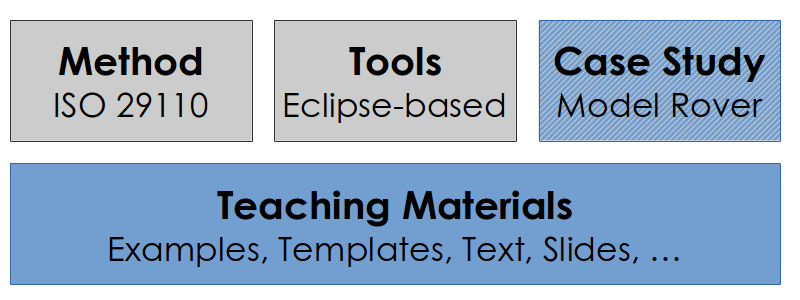
\includegraphics[width=\textwidth]{../se-images/teaching-overview.png}
  \caption{Scope of the SE teaching materials}
  \label{fig:scope}
\end{figure}

%-------------------------------------------------------------------------------
\subsection{Software vs. Systems Engineering}
%-------------------------------------------------------------------------------

For the purpose of this tutorial, a system has interfaces with other software or hardware, while software is (more or less) stand-alone.  Using this definition, we see systems engineering simply as an extension to software engineering, but with interfaces that can be unreliable.

%-------------------------------------------------------------------------------
\subsection{Standards}
%-------------------------------------------------------------------------------

ISO 29110 looks promising as the foundation for the method. Eclipse-based tools in general, and ProR for requirements engineering in particular, will be used. We are currently looking for a suitable case study, ideally using something that already exists. The focus will be on the creation of shared teaching materials. 
%-------------------------------------------------------------------------------

%===============================================================================
\section{Tools}
%===============================================================================

A central idea of this project is the use of freely available tools, as we cannot expect students to invest in expensive tools.  Tools will be based on Eclipse.  Figure~\ref{fig:v-model} shows on the left a simplified V-Model, depicting the tools we plan to use.

\begin{figure}[h!]
  \centering
  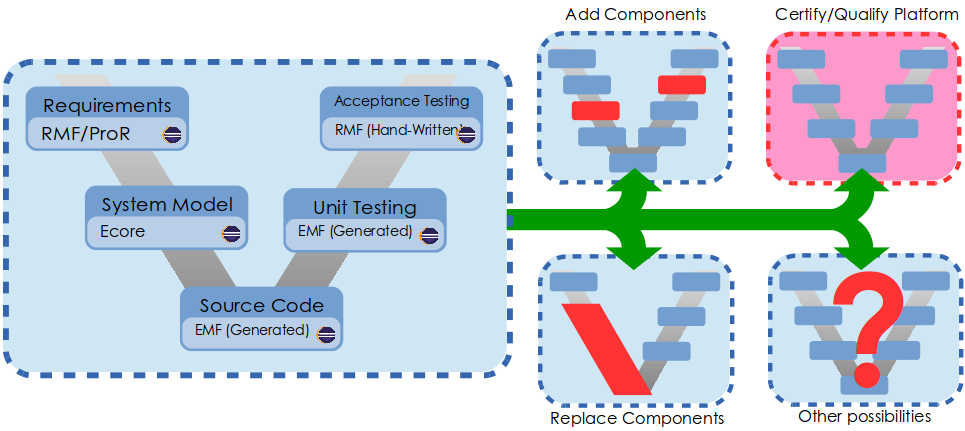
\includegraphics[width=\textwidth]{../se-images/toolchain.pdf}
  \caption{Tools used in this course}
  \label{fig:v-model}
\end{figure}

\begin{info}
In a ``real'' project, there would be many more tools and artifacts.  We will keep tools and artifacts to a minimum, in order not to overwhelm the students.
\end{info}

As you can see, we plan on building a \textbf{minimal, complete, Eclipse-based} software engineering platform.  It is loosely organized according to the V-Model.

%-------------------------------------------------------------------------------
\subsection{Modularity and Extendability}
%-------------------------------------------------------------------------------

Figure~\ref{fig:v-model} depicts on the right how this toolchain can be adapted to your needs.


Openness helps drastically to make this possible:

\begin{description}
\item[Open Standards] make it possible to replace individual tool components, without disturbing the toolchain as a whole.  Open Standards that we use include ReqIF, Java and JUnit.
\item[Open Software] allows the toolchain to be tailored and seamlessly integrated in a way that is very difficult to do otherwise.
\end{description}

%===============================================================================
\section{Background}
%===============================================================================

This project started in July 2014 as a discussion on \href{https://www.linkedin.com/groupItem?commentID=-1&item=5890782095432781827&type=member&gid=128312&view=}{LinkedIn}.  Thank you to all contributors!

%===============================================================================
\section{License}
%===============================================================================

This content is licensed as Apache 2.0.  If you contribute to the corresponding gitHub repository, you implicitly license the content that way.




\chapter{Tutorial}
This chapter contains a mini-tutorial that has been used by Michael Jastram for the TdSE 2014 talk \href{http://www.tdse.org/programm2013/termine/icalrepeat.detail/2014/11/12/83/-/t2-modellgetriebene-systementwicklung-mit-eclipse.html}{Modellgetriebene Systementwicklung mit Eclipse}.

% ==================================================================
\section{Overview}
% ==================================================================

This tutorial covers the development of a small traffic light system, as shown in Figure~\ref{fig:trafficlight}.

\begin{figure}[h!]
  \centering
  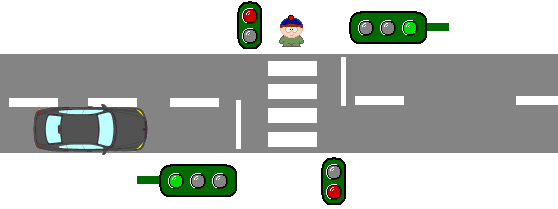
\includegraphics[width=0.8\linewidth]{../se-images/trafficlight.png}
  \caption{We will model a simple traffic light system.}
  \label{fig:trafficlight}
\end{figure}

% ==================================================================
\section{Tool Installation}
\label{sec:tutorial-tool-installation}
% ==================================================================

As of this writing, a complete toolchain is not yet available.  The following describes the installation from various components.

% ------------------------------------------------------------------
\subsection{Eclipse}
% ------------------------------------------------------------------

The basis for the toolchain are the \href{https://www.eclipse.org/downloads/packages/eclipse-modeling-tools/lunasr1}{Eclipse Modeling Tools}.  Please download for your platform and extract to a convenient location and start it.

\begin{info}
It may be not a bad idea to start with Polarsys instead, as it already includes Papyrus.
\end{info}

\begin{warning}On Linux, please edit eclipse.ini and add the following parameter \textbf{at the top (two lines}):

\begin{lstlisting}
--launcher.GTK_version
2
\end{lstlisting}
\end{warning}

% ------------------------------------------------------------------
\subsection{RMF and Formal Mind Essentials}
% ------------------------------------------------------------------

Next install the RMF (requirements) tools, but the repackaged version from Formal Mind:

\begin{itemize}
\item Use this update site: http://update.formalmind.com/studio
\item Unselect ``Group items by category''
\item Select \textbf{only} ``Formal Mind Studio (Feature)''
\item Complete the installation.
\end{itemize}

\begin{info}
The software is currently not signed, which will generate a warning.  Please continue with the installation, in spite of this.
\end{info}

% ------------------------------------------------------------------
\subsection{Java FX}
% ------------------------------------------------------------------

If you want to use rich text in requirements, you need support for Java FX.  Follow these steps:

\begin{itemize}
\item Use this update site: http://download.eclipse.org/efxclipse/runtime-released/1.1.0/site
\item Optional: Unselect ``Group items by category''
\item Select \textbf{only} ``Runtime Bundle Collector Feature''
\item Complete the installation.
\end{itemize}

% ------------------------------------------------------------------
\subsection{RMF-EMF Traceability}
% ------------------------------------------------------------------

In the context of a public research project (itea openETCS), a traceability plug-in for connecting arbitrary EMF models has been developed.

\begin{itemize}
\item Use this update site: http://openetcs.ci.cloudbees.com/job/openETCS-tycho/lastSuccessfulBuild/artifact/tool/bundles/org.openetcs.releng.products/target/repository
\item Unselect ``Group items by category''
\item Select \textbf{only} ``ProR Tracing Feature''
\item Complete the installation.
\end{itemize}

% ------------------------------------------------------------------
\subsection{Additional Modeling Components}
% ------------------------------------------------------------------

You can install additional components for modeling via \menu{Papyrus via Help | Install Modeling Components}.  For this tutorial, useful components include:

\begin{description}
\item[Ecore Tools.] Support diagram notation for Ecore models.
\item[Papyrus.] Supports UML and SysML.
\end{description}

We had some problems with installing the Ecore Tools.  If you cannot see a diagram in Section~\ref{}, then follow these steps:

Install software from this update site: http://download.eclipse.org/ecoretools/updates/releases/2.0.1/luna
Select Ecore Diagram Editor

% ------------------------------------------------------------------
\subsection{Team Support}
% ------------------------------------------------------------------

Eclipse supports a number of team environments.  We recommend the installation of the egit plugin, allowing to work with git repositories.  The installation is described in the \href{http://formalmind.com/handbook?page=sec-versioning.html}{formalmind Studio Handbook}.

% ------------------------------------------------------------------
\subsection{Tool Configuration}
% ------------------------------------------------------------------

We recommend to switch to the ProR perspective, to get started.

% ==================================================================
\section{Import Requirements}
\label{sec:tutorial-import}
% ==================================================================

Typically, you already have requirements available in some form.  ProR includes a simple CSV-Importer that allows you to import existing requirements.  Follow these steps:

\begin{itemize}
\item Create a new Project via \menu{File | New | Project... | General | Project}
\item Call it \menu{tdse-1}
\item Create a new Requirements Model via right-click on the project, selecting \menu{New | Reqif10 Model}
\item Call the Model \menu{Trafficlight.reqif}
\item Import the .csv file via \menu{File | Import | formalmind Studio | CSV}
\item Create a mapping for the two columns to String attributes, as shown in Figure~\ref{fig:csv-import}
\end{itemize}

\begin{figure}[h!]
  \centering
  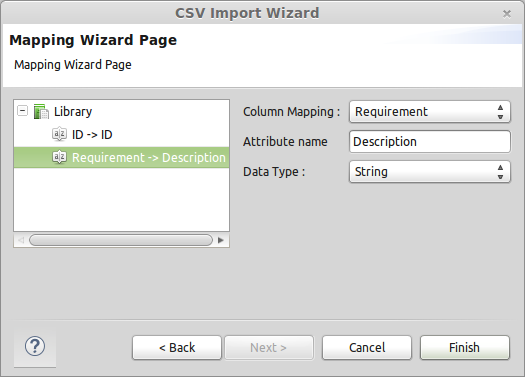
\includegraphics[width=0.8\linewidth]{../se-images/csv-import.png}
  \caption{Result: The requirement is now a sibling of the chosen requirement.}
  \label{fig:csv-import}
\end{figure}

After the import, the new requirements have been added to the existing requirements specification.  There are a number of recommended improvements, for instance:

\begin{itemize}
\item Add a SpecObjectType for Headlines and configure the Headline Presentation, so that you can structure the text
\item Once you create headlines, you can arrange requirements as child elements (instead of siblings) under them.
\item You can create an information SpecObjectType, using XHTML and no IDs.  Use one of these to insert Figure~\ref{fig:trafficlight} into your specification (\href{../se-materials/tutorial/trafficlight.png}{trafficlight.png}).
\item Configure the ID Presentation to automatically create IDs for requirements, and center-align the ID.
\item Use the ID as a label (if available) by adjusting the Label Configuration.
\end{itemize}

The resulting specification is shown in Figure~\ref{fig:tutorial-step01}.

\begin{figure}[h!]
  \centering
  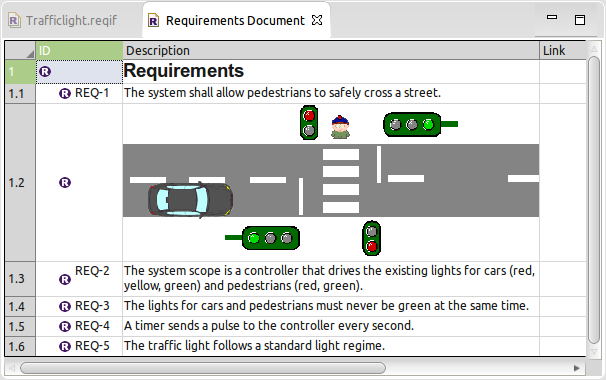
\includegraphics[width=\linewidth]{../se-images/tutorial-step01.png}
  \caption{The spec after completion of all steps so far.}
  \label{fig:tutorial-step01}
\end{figure}

% ==================================================================
\section{Glossary}
\label{sec:tutorial-glossary}
% ==================================================================

A glossary helps keeping track of terminology.  In this section, the glossary management from formalmind Studio is introduced, which supports color highlighting in the requirements text.

Note that this kind of glossary is a ``dead end'', in the sense that it cannot be used beyond its purpose.  Contrast that with a model-based data dictionary, as described in Section~\ref{sec:tutorial-ecore}.

The glossary is kind of cumbersome to configure.   Therefore, we included a correctly configured \href{../se-materials/tutorial/tdse-2/}{Sample Project}.  Note that you need both the Highlighting and Keyword Highlighting presentations, in that order.

Figure~\ref{fig:tutorial-step02} shows the glossary, and its application to the requirements, which have been rewritten to use the terminology of the specification.

\begin{figure}[h!]
  \centering
  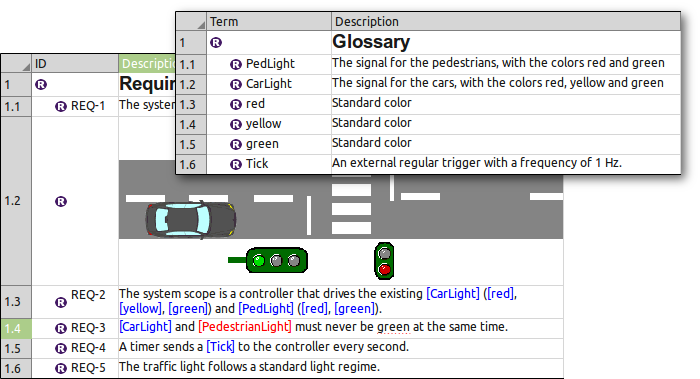
\includegraphics[width=\linewidth]{../se-images/tutorial-step02.png}
  \caption{Glossary Management in action.}
  \label{fig:tutorial-step02}
\end{figure}

In the screenshot, REQ-3 is being edited.  This results in the word \textit{green} being underlined in red, indicating that it is a recognized glossary entry.  The syntax highlighting diapears when not in edit mode.  Square brackets make a glossary term explicit.  If a term is marked that way that is not in the glossary, then it is shown in red.

% ==================================================================
\section{Data Dictionary with Ecore}
\label{sec:tutorial-ecore}
% ==================================================================

Ecore is the modeling language of the Eclipse Modeling Framework.  It has some similarities to UML Class diagrams, and is therefore well-suited for creating a precise data model.  It has the following advantages:

\begin{description}
\item[Easy to learn.] Especially if you already know class diagrams, you should be able to quickly learn Ecore.
\item[Code generation.] EMF allow the generation of Java code from Ecore models.  You can even generate a GUI based on a tree view.
\item[Test stub generation.] EMF allows the generation of test code stubs, making it easy to cover the unit test level.
\end{description}

On the other hand, it has its limitations.  In particular, it is not really possible to model dynamic aspects of the system.

\begin{warning}
While it is possible to mix this approach with the glossary management described in Section~\ref{sec:tutorial-glossary}, we do not recommend it, as it would lead to redundancy.  Redundancies should be avoided (DRY-principle: Don't Repeat Yourself).
\end{warning}

% ------------------------------------------------------------------
\subsection{Creating the Ecore Model}
% ------------------------------------------------------------------

We recommend to create a new Ecore Modeling Project via \menu{File | New | Project... | Eclipse Modeling Framework | Ecore Modeling Project}.   This way, everything will be properly configured for code generation and other cool stuff.  The model we use is shown in the right pane of Figure~\ref{fig:tutorial-step03}.

\begin{figure}[h!]
  \centering
  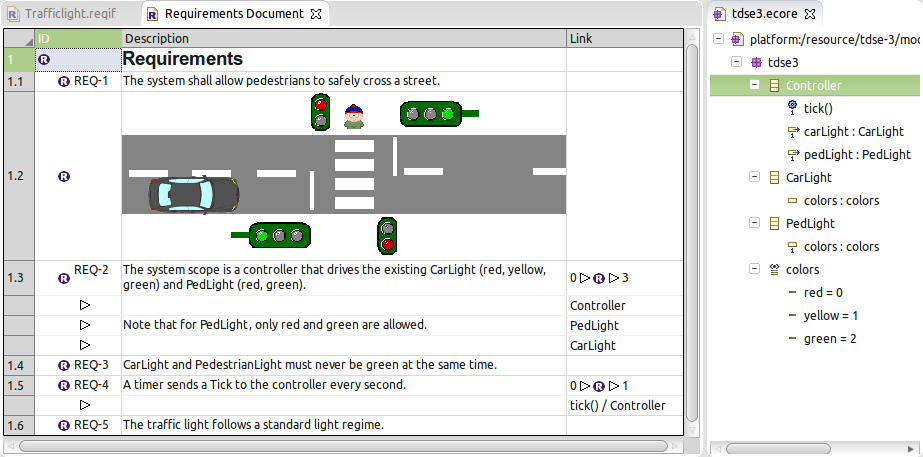
\includegraphics[width=\linewidth]{../se-images/tutorial-step03.png}
  \caption{On the left the requirements with links into the Ecore-based data model, shown on the right.}
  \label{fig:tutorial-step03}
\end{figure}

As you can see, the editors are arranged so that the requirements editor and the Ecore editor are visible at the same time.  This is necessary, as links are created by dragging model elements from the Ecore model onto the requirements.

\begin{info}
Linking via Drag and Drop is a feature taken from the openETCS project, \href{https://github.com/openETCS/toolchain/wiki/User-Documentation#Tracing_Requirements_and_SysML_Models}{where it is documented}.
\end{info}

We provided a preconfigured \href{../se-materials/tutorial/tdse-3/}{Sample Project}, that allows annotating traces, as also shown in Figure~\ref{fig:tutorial-step03} (the second link of REQ-2).

% ------------------------------------------------------------------
\subsection{Working with Diagrams}
% ------------------------------------------------------------------

Some people prefer diagrams to the tree-view shown in Figure~\ref{fig:tutorial-step03}, and diagrams can make communication easier.  If you installed the tool as described in Section~\ref{sec:tutorial-tool-installation}, then you can create a diagram from the Ecore model as described here.  Diagram and model will be synchronized, but it's possible to only show a subset of the model elements in the diagram.

A diagram should already have been created upon project creation.  You can open it by going to the Model Explorer or Project Explorer, and opening the .ecore model by clicking on the \[+\] to the left of the file name. it should show the package name (tdse3), and upon opening it again, it should unveal ``tdse3 class diagram''.  Doubleclicking should open the diagram editor, which will be empty, except instructions on how to add elements.

\begin{figure}[h!]
  \centering
  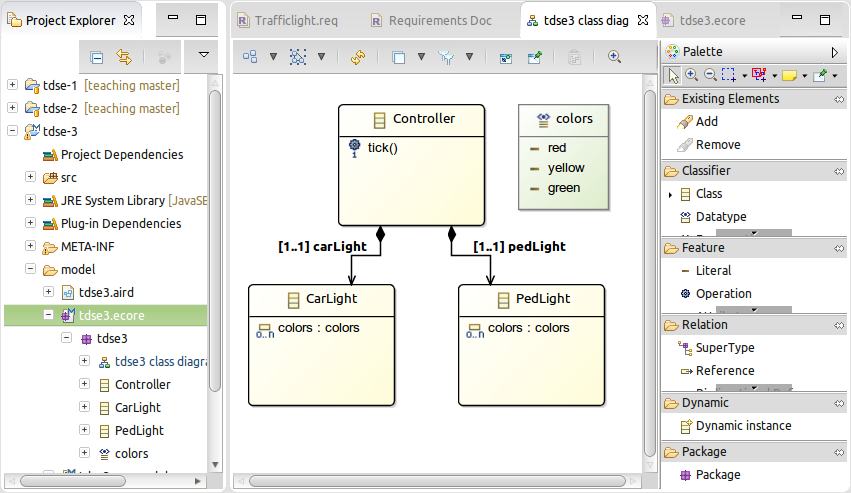
\includegraphics[width=\linewidth]{../se-images/ecore_diagram.png}
  \caption{The diagram has been created by dragging elements from the Project Explorer (left) to the drawing area (middle).  New elements can also be created by using the pallet on the right.}
  \label{fig:ecore_diagram}
\end{figure}

By dragging elements from the project explorer into the diagram area, we end up with the editor, as shown in Figure~\ref{fig:ecore_diagram}.  Elements and labels can be customized as one sees fit.  Changes to the model, including the creation of new elements, will be reflected in the tree view of the Ecore model as well.  Changes to the Ecore model will be seen here, but newly created elements will not appear on the diagram by default.  They have to be added manually.

% ==================================================================
\section{Traceability}
% ==================================================================

In the previous section, we saw for the first time links (or traces) in ProR.  Traces are useful for many things, including change management.

Traces can are typed and can have an arbitrary number of attributes.  In ProR, traces can be created via drag and drop, or via context menu.  The latter is recommended, as it makes it easy to link multiple requirements at the same time, and allows to set the type with one click, as shown in Figure~\ref{fig:linking-finish}.

\begin{figure}[h!]
  \centering
  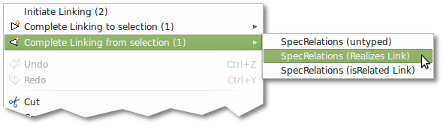
\includegraphics[width=0.6\linewidth]{../se-images/linking-finish.png}
  \caption{Completing a link operation.}
  \label{fig:linking-finish}
\end{figure}

\begin{info}
We wrote an article in the \href{http://formalmind.com/de/blog/better-link-creation-rmf-pror-070}{Formal Mind Blog} on how to create links in detail.
\end{info}

% ------------------------------------------------------------------
\subsection{Change Management}
% ------------------------------------------------------------------

With change management, you want to know if a relationship has to be re-evaluated.  There is a free extension available for this purpose, as part of the Formal Mind Essentials (which should be installed, if you followed the installation instructions).  With this extension, two flags on the link are set if source or target change, respectively.  This is shown in Figure~\ref{fig:change-mgmt}.

\begin{figure}[h!]
  \centering
  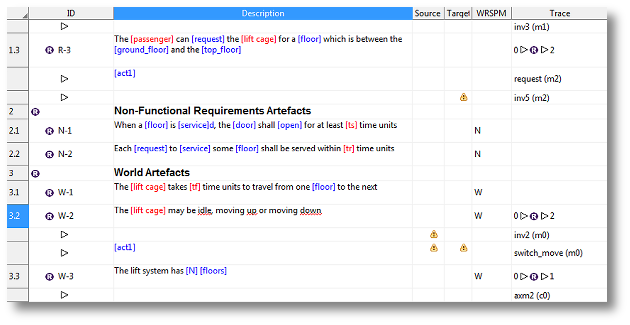
\includegraphics[width=0.8\linewidth]{../se-images/ProRArtefacts_Trace_LL.png}
  \caption{When source or target of a link change, a corresponding flag is set on the link.}
  \label{fig:change-mgmt}
\end{figure}

This mechanism also works with external models, e.g. the traceability the the Ecore model that was described in Section~\ref{sec:tutorial-ecore}.

% ==================================================================
\section{Modeling with SysML and Papyrus}
% ==================================================================

An alternative to the RMF/Ecore approach is to use SysML with Papyrus.  SysML has a requirements type, which would allow covering requirements and model in one overarching model.  Further, SysML contains Sequence Diagrams, Activity Diagrams and State Machines, thereby supporting the modeling of dynamic behavior as well.

To use SysML, create a SysML Project via \menu{File | New | Project... | Papyrus | SysML Project}. When asked for the diagrams to be created, sselect the ``Block Definition Diagram'' (roughly equivalent to a Class Diagram) and the ``Requirements Diagram''.

We will explore this further in the future, but consider SysML to be overkill at this point.

% ==================================================================
\section{Code Generation with Ecore}
% ==================================================================

The Ecore model we created in Section~\ref{sec:tutorial-ecore} can be used to generate a number of different pieces of code, by default Java:

\begin{description}
\item[Model Code.] This is fairly simple code that manages getters and setters, relationships, persistence, notifications, etc.
\item[GUI Code.] This consists of an ``Edit'' model that can drive a user interface, but does not contain GUI code itself.  A simple reflective user interface can be created as well, which looks very much like the Tree-based Ecore editor.
\item[Test Code.] The framework generates stubs for unit tests, which have to be implemented manually.
\end{description}

The generation is driven by a ``Generator Model'', which has already been created when we built the Ecore model.  It resides in the same folder.

% ------------------------------------------------------------------
\subsection{Model Code}
% ------------------------------------------------------------------

We generate the Model code via Right-Click on the top-level element of the generator model and select \menu{Generate Model Code}.

The code will be generated in the same project.  Let's implement a little program for testing:
\begin{lstlisting}
public static void main(String[] args) {
	Controller controller = Tdse3Factory.eINSTANCE.createController();
	while (true) {
		print(controller);
		controller.tick();
	}
}

private static void print(Controller controller) {
	System.out.println("cars: " + controller.getCarLight().getColors() +
			"peds: " + controller.getPedLight().getColors());
}
\end{lstlisting}

Of course, this program will not run as is: the lights will be null, the method tick() has not been implemented, etc.  This is left as an exercise to the reader.

% ==================================================================
\section{Unit Testing}
% ==================================================================

Similar to the generation of the model code, you can generate stubs for unit tests. Right-Click on the top-level element of the generator model and select \menu{Generate Model Code}.

By default, the test code is created in a separate project.  The inheritance hierarchy of the test classes reflects those of the model.  Each class sets up and tears down a ``fixture'', an instance of the class under test.

Tests are also inherited: If you implement a test for a superclass in the corresponding unit test file, using the fixture, then the same test will be executed for the derived classes as well.

% ------------------------------------------------------------------
\subsection{Mocking}
% ------------------------------------------------------------------

Even at the unit test level, you may be confronted with the fact that the ``real'' thing to be tested is not available.  This is particularly relevant for systems.  Consider a software system, for instance, that relies on a web API to operate.  On the unit test level, you would typically not want to communicate with the real API.  It would be hard to determine whether the API is down or the test broken.

The solution for this is ``mocking'': Writing code that mimics the real thing, but only those aspects relevant for the test.  Conveniently, mocking also allows testing a service that misbehaves, allowing fault and error conditions to be tested as well.

There is a wide array of mocking frameworks available.  We had good experience with JMockit, but there are many others.

% ------------------------------------------------------------------
\subsection{Functional and Integration Testing}
% ------------------------------------------------------------------

For the scope covered in this document, there is nothing between unit tests and acceptance tests.  But in any project of non-trivial size, and in particular for systems engineering projects, there are functional and integration tests.

If a test can be automated, then it can typically still be realized by leveraging JUnit.  In particular, an integration test can be quite similar to a unit test, except that it does not use mocking, but ``the real thing''.  This can be an API of a service that is called in real time, or it can be real hardware that responds.

\begin{figure}[h!]
  \centering
  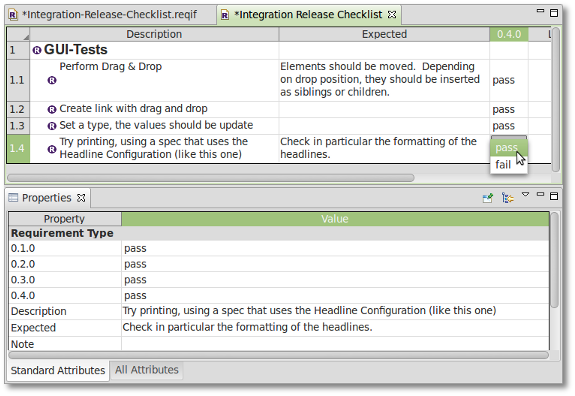
\includegraphics[width=\linewidth]{../se-images/manual-testing-1.png}
  \caption{The diagram has been created by dragging elements from the Project Explorer (left) to the drawing area (middle).  New elements can also be created by using the pallet on the right.}
  \label{fig:manual-testing}
\end{figure}

% ==================================================================
\section{Acceptance Testing}
% ==================================================================

With acceptance testing, we reach the top of the V again.  Acceptance tests are hard to automate.  There may be scenarios where it is possible, and then some techniques from the previous section could be employed.  But more often than not, they have to be performed manually.  In this section, we use ProR/RMF again to implement manual testing.

\begin{info}
There is a more elaborate description of this technique in the \href{http://formalmind.com/de/blog/manual-testing-pror}{Formal Mind Blog}
\end{info}

% ------------------------------------------------------------------
\subsection{A Test Result Specification}
% ------------------------------------------------------------------
Tests are defined in a separate document that is part of the same .reqif file.  Corresponding to Section~\ref{sec:tutorial-import}, the document can be styled with headlines, sections, etc.

But the important thing is to create an enumeration data type for recording the tests results, typically ``pass'' and ``fail''.

When the time comes to run a test, the tester creates a new attribute for the version under test.  Now, each test can be performed, and the result recorded, as shown in Figure~\ref{fig:manual-testing}.

The nice thing is, that old tests will be preserved.  The main view (Specification Editor) can be configured to only show the version of interest, but in the properties view, all past test results are still there to be inspected.



%\chapter{Case Study}
%We have not decided on a case study yet.  Candidates so far are:

\begin{description}
\item[Coffee Maker.] A long-time favorite, and there are at least three available
\item[FAA Isolette.] This is a complete example from a safety-critical domain. 
\item[Rover.] This one is driven by Gaël Blondelle from the Eclipse Foundation. On the plus side, it's great for the classroom, as the hardware is cheap. But in contrast to the others, there is nothing there yet. 
\end{description}

Teaching Materials can be made available via \href{../se-materials/Example.reqif}{relative links}.


\end{document}

